%Copyright (c) 2004 2005 2006 Atos Origin
%Permission is granted to copy, distribute and/or modify this
%document
%under the terms of the GNU Free Documentation License,
%      Version 1.2
%      or any later version published by the Free Software
%      Foundation;
%      with no Invariant Sections, no Front-Cover
%      Texts, and no Back-Cover
%      Texts.  A copy of the license is
%      included in the section entitled "GNU
%      Free Documentation License".
%
% $Id: qsos.tex,v 1.3 2006/03/09 09:34:40 goneri Exp $
\documentclass[a4paper]{article}

\usepackage[T1]{fontenc}      % Police contenant les caract�res fran�ais ? No need in english ?
\usepackage{geometry}         % D�finir les marges
\usepackage[spanish]{babel}  % Placez ici une liste de langues, la
\usepackage{hyperref}
\usepackage{graphicx}  % picture incusion 
\usepackage{url}
\usepackage{color}
\usepackage{fancyhdr}
\pagestyle{fancy}
\usepackage{float}
%\floatstyle{ruled}
%\newfloat{figure}{thp}{lop}
\newfloat{figure}{!htb}{lop}
\floatname{figure}

\date{January 2006}
\author{}
\title{Method for Qualification and Selection \\ of Open Source software (QSOS) \\ version 1.5}
% title param :  title, author, date
\begin{document}

\cfoot{}
\rfoot{Page \thepage{}}
\lfoot{{\footnotesize \textbf{QSOS 1.5} Copyright \copyright 2004,2005,2006 Atos Origin\\
Document under the terms of the Gnu FDL \url{http://www.gnu.org/copyleft/fdl.html}}}
\renewcommand{\footrulewidth}{0.5pt}

\renewcommand{\arraystretch}{1.75} 
\setlength{\tabcolsep}{10pt}

% MACRO
% TabluarStrong : for tabular colonne title
\newcommand{\TS}[1]{\textbf{#1}}

% Begin of the document
\maketitle

\begin{figure}
\center
\includegraphics[width=13cm]{images/QSOS}
\end{figure}


\begin{abstract}
\begin{center}
This document describes the QSOS method, conceived to qualify, select and compare free and open source software in an objective, traceable and argued way.


It is made available to all, under the terms of the \\ \textbf{GNU Free Documentation Licence}.


This document and its \LaTeX\ source files are available on \textbf{\url{http://www.qsos.org}}.
\end{center}
\end{abstract}

\newpage
\tableofcontents

%Copyright (c) 2004 2005 2006 Atos Origin
%Permission is granted to copy, distribute and/or modify this
%document
%under the terms of the GNU Free Documentation License,
%      Version 1.2
%      or any later version published by the Free Software
%      Foundation;
%      with no Invariant Sections, no Front-Cover
%      Texts, and no Back-Cover
%      Texts.  A copy of the license is
%      included in the section entitled "GNU
%      Free Documentation License".
%
%$Id: license.tex,v 1.1 2006/02/16 18:21:09 goneri Exp $
\section{Note de licence}

Copyright \copyright 2004, 2005, 2006 Atos Origin


Vous pouvez copier, redistribuer et/ou modifier ce document selon les termes de la Licence de Documentation
Libre GNU, Version 1.2 publi�e par la Free Software Foundation ; la Section Invariante �tant "Manifeste
QSOS", le Texte de Premi�re de Couverture �tant : "Ce document ainsi que ses fichiers source \LaTeX\ sont disponibles sur \url{http://www.qsos.org}", et aucun Texte de Quatri�me de Couverture. Une copie de la licence en
langue anglaise est consultable sur le site
\url{http://www.gnu.org/copyleft/fdl.html}, une traduction
fran�aise non officielle est consultable sur le site Web de Wikipedia (\url{http://fr.wikipedia.org/wiki/FDL}).


La licence s'applique �galement aux documents g�n�r�s par l'application de la m�thode, � savoir les grilles fonctionnelles, les fiches d'identit� et les fiches d'�valuation pr�sent�es dans la section "�valuer".

%Copyright (c) 2004 2005 2006 Atos Origin
%Permission is granted to copy, distribute and/or modify this
%document
%under the terms of the GNU Free Documentation License,
%      Version 1.2
%      or any later version published by the Free Software
%      Foundation;
%      with no Invariant Sections, no Front-Cover
%      Texts, and no Back-Cover
%      Texts.  A copy of the license is
%      included in the section entitled "GNU
%      Free Documentation License".
%
%$Id: manifest.tex,v 1.1 2006/02/16 16:33:33 goneri Exp $
\section{The QSOS Manifesto}

\subsection{Why a method?}
For a company, the choice to opt for a software as component of its information
system, wether this software is Open Source or commercial, rests on the
analysis of needs and constraints (technical, functional and strategic) and on the adequacy 
of the software to these needs and constraints 

However, when one plans to study the adequacy of open source software, it is necessary to have 
a method of qualification and selection adapted to peculiarities of this type of software. 
It is, for instance, particularly important to precisely examine the constraints and risks 
specific to open source software. 
Since the open source field is very rich and has a very broad scope, it is also 
necessary to use a qualification method allowing to
differentiate the quite often numerous candidates to meet both technical, functionnal and strategic requirements.

Beside "natural" questions like:
\begin{itemize}
\item Which software meets best my actual/planned {\bf technical} requirements?
\item Which software meets best my actual/planned {\bf functional} requirements?
\end{itemize}

Here some questions every company should answer before making any decision:
\begin{itemize}
\item What is the durability of the software? What are the risks of Forks? How to anticipate and manage them?
\item What level of stability to expect? How to manage dysfunctions?
\item What is expected and available support level provided on the software?
\item Is it possible to have influence on the software (addition of new or specific functionalities)?
\end{itemize}


To be able to answer serenely this type of questioning and thus set up an
efficient risk management, it is imperative to have a method allowing:
\begin{itemize}
\item to qualify software by integrating the open source peculiarities;
\item to compare several software according to formalized needs requirement of weighted criteria, in order to carry out a final choice.
\end{itemize}

These are the various points which made Atos Origin to conceive and formalize the method for Qualification and Selection of Open Source software (QSOS).


\subsection{Why a free method?}
For us, such a method as well as the results it generates, must be made available to all under the terms of a free licence. Only such a licence is capable to ensure the promotion of the open source movement, via in particular:
\begin{itemize}
\item the ability for all to re-use already available work of qualification and evaluation;
\item the quality and objectivity of documents generated, always perfectible according to principles of transparency and
peers review.
\end{itemize}
For these reasons Atos Origin decided to make available the QSOS method, and the documents generated during its application (functional grids, identity cards and evaluation sheets), under the terms of the GNU Free Documentation License.

%Copyright (c) 2004 2005 2006 Atos Origin 
%Permission is granted to copy, distribute and/or modify this
%document
%under the terms of the GNU Free Documentation License,
%      Version 1.2
%      or any later version published by the Free Software
%      Foundation;
%      with no Invariant Sections, no Front-Cover
%      Texts, and no Back-Cover
%      Texts.  A copy of the license is
%      included in the section entitled "GNU
%      Free Documentation License".
%$Id: changelog.tex,v 1.1 2006/02/16 17:36:15 goneri Exp $
\section{Changelog}
\begin{figure}
\center
\begin{tabular}{|p{1.5cm}|p{1.7cm}|p{3cm}|p{5.6cm}|}
\hline \TS{Version} & \TS{Date} & \TS{Authors} & \TS{Comments}\\
\hline \TS{1.0} & & Rapha�l SEMETEYS (Atos Origin) & Initial conception and redaction.\\
\hline \TS{1.1} & & Olivier PILOT (Atos Origin) & Conception and proofreading.\\
\hline \TS{1.2} & & Laurent BAUDRILLARD (Atos Origin) & Conception and proofreading.\\
\hline \TS{1.3} & \date{17/11/2004} & Rapha�l SEMETEYS (Atos Origin) & First official release.\\
\hline \TS{1.4} & \date{23/11/2005} & Rapha�l SEMETEYS (Atos Origin) & Corrections of misprints, addition of the "License notice" and "Changelog" sections.

Replacement of the evaluation example by a link to \url{http://www.qsos.org}.\\
\cline{3-4} & & Olivier PILOT (Atos Origin) & New logo.\\
\hline \TS{1.5} & \date{19/01/2006} & Gon�ri LE BOUDER (Atos Origin) &

Conversion to \LaTeX\ .

Re-licensing under the Gnu FDL.\\

\cline{3-4} & & Rapha�l SEMETEYS (Atos Origin) & Addition of the "QSOS Manifesto" section.


First english version.\\
\hline
\end{tabular}
\end{figure}


%Copyright (c) 2004 2005 2006 Atos Origin
%Permission is granted to copy, distribute and/or modify this
%document
%under the terms of the GNU Free Documentation License,
%      Version 1.2
%      or any later version published by the Free Software
%      Foundation;
%      with no Invariant Sections, no Front-Cover
%      Texts, and no Back-Cover
%      Texts.  A copy of the license is
%      included in the section entitled "GNU
%      Free Documentation License".
%
%$Id: intro.tex,v 1.1 2006/02/16 17:36:15 goneri Exp $
\section{Introduction}

\subsection{Document objective}
This document describes the QSOS method (Qualification and Selection of software Open Source), conceived by Atos Origin to qualify and select the Free and Open Source software as a basis of its support and technological survey services.

The method can be integrated within a more general process of technological survey which is not presented here. It describes a process to set up identity cards and evaluation sheets for free and open source software.

\subsection{Targeted readers}
This documlent targets the following readers:
\begin{itemize}
\item people curious to know more about the method, on a professional or personnal basis;
\item communities of Free and Open Source projects;
\item IT experts wishing to know and use the method in their task of evaluating and selecting of components to build systems for their own needs or for their customers.
\end{itemize}



%Copyright (c) 2004 2005 2006 Atos Origin
%Permission is granted to copy, distribute and/or modify this
%document
%under the terms of the GNU Free Documentation License,
%      Version 1.2
%      or any later version published by the Free Software
%      Foundation;
%      with no Invariant Sections, no Front-Cover
%      Texts, and no Back-Cover
%      Texts.  A copy of the license is
%      included in the section entitled "GNU
%      Free Documentation License".
%
%$Id: general_process.tex,v 1.1 2006/02/16 17:36:15 goneri Exp $
\section{General process}
\subsection{Four steps}
The general process of QSOS is made up of several interdependent steps (figure~\ref{fig-process}).

\begin{figure}[h]
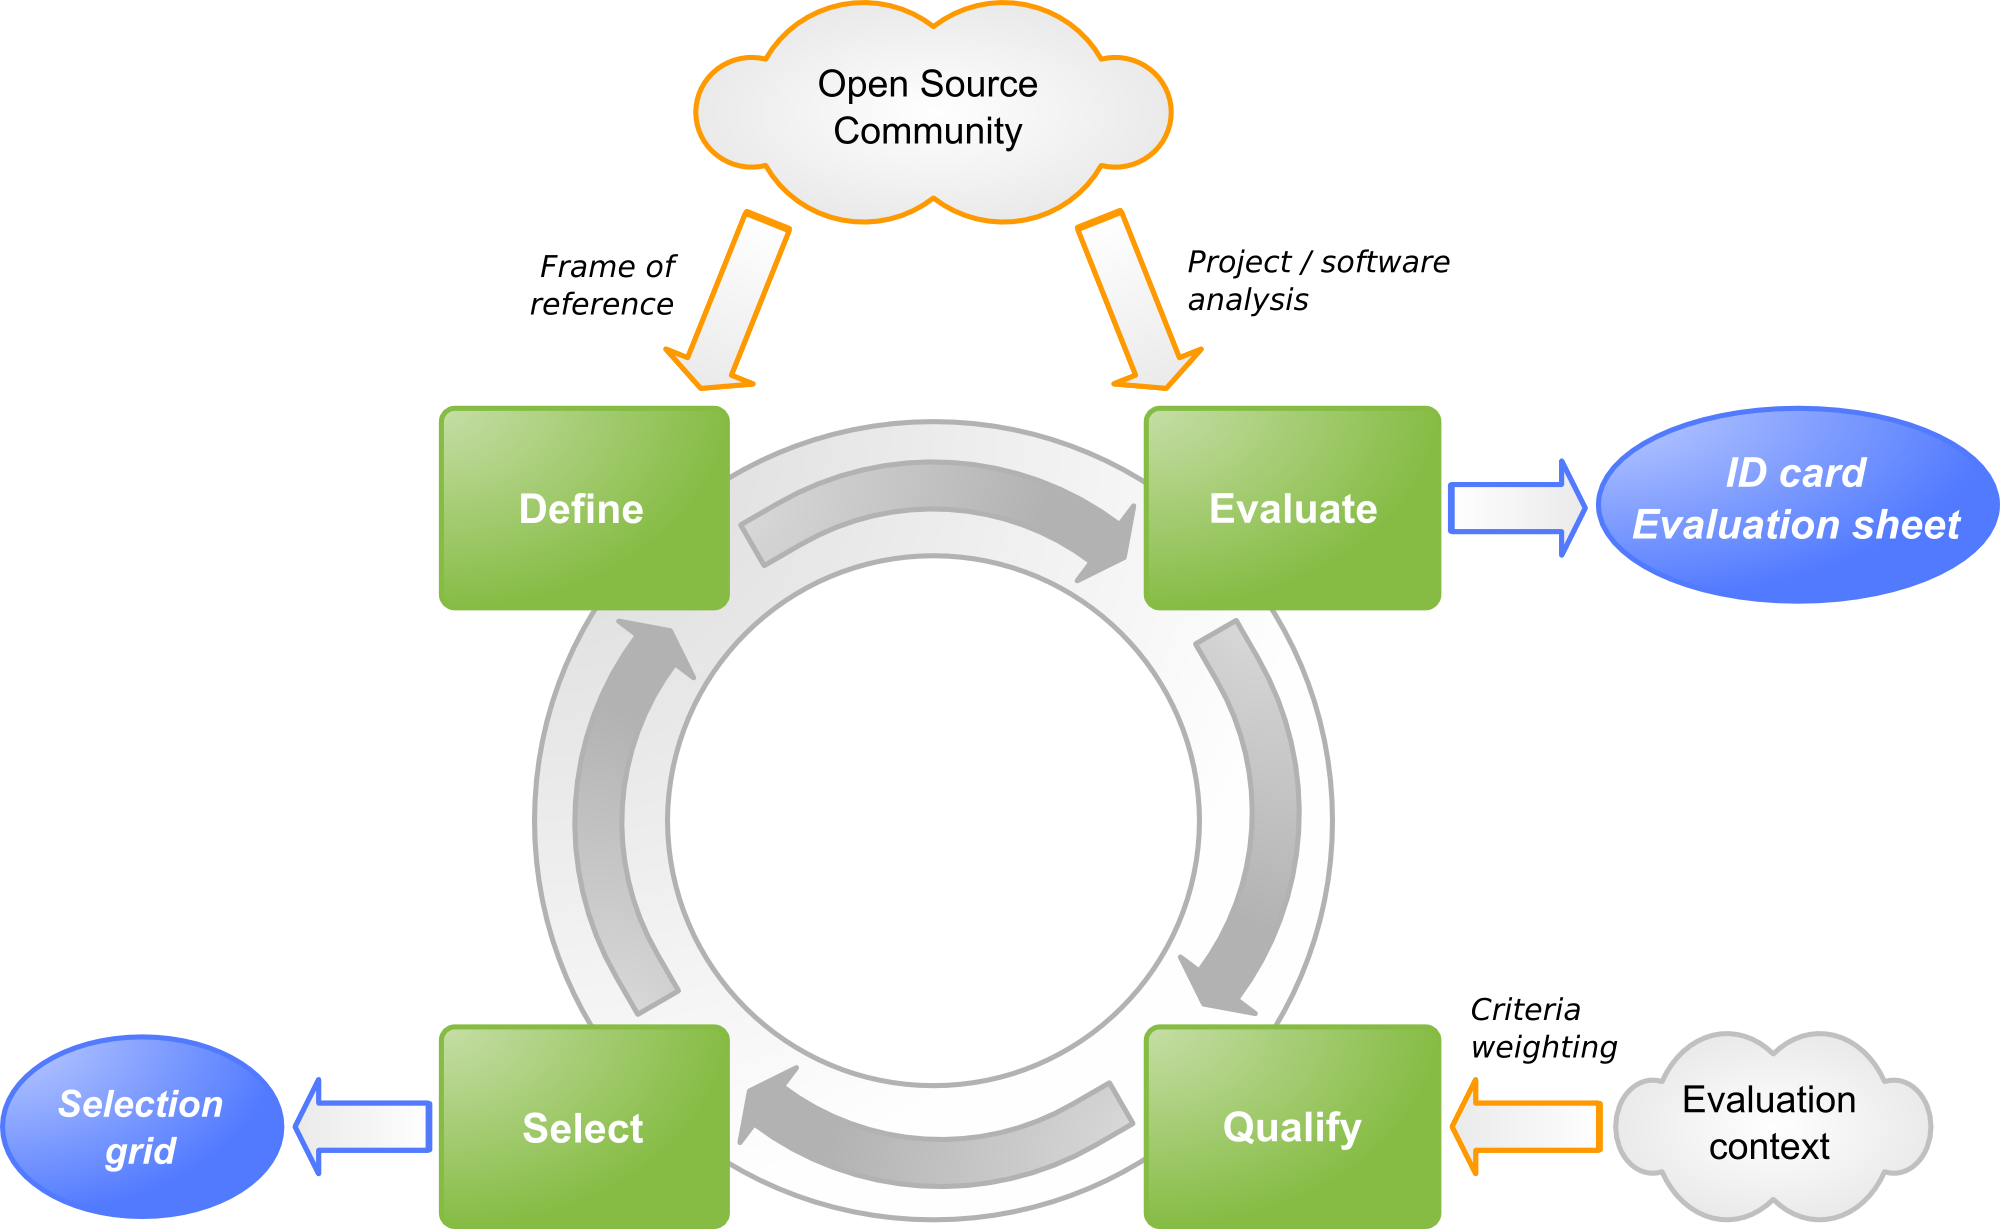
\includegraphics[width=16cm]{images/processus_4_etapes}
\caption{The 4 steps of QSOS}
\label{fig-process}
\end{figure}

\begin{figure}
%a faire en mieux
\center
\begin{tabular}{|p{3cm}|p{9cm}|}
\hline \TS{Step} & \TS{Description}\\
\hline 1 - Define & Constitution and enrichment of frames of reference used by following steps.\\
\hline 2 - Evaluate & Evaluation of software made on three axis of criteria: functional coverage, risks for the user and risks for the service provider (independently of any particular user/customer context).\\
\hline 3 - Qualify & Weighting of the criteria split up on the three axes, modeling the context (user requirements and/or strategy set by the service provider).\\
\hline 4 - Select & Application of the filter set up in Step 3 - "Qualify" on data provided by the first two steps, in order to proceed queries, comparisons and selections of products.\\
\hline
\end{tabular}
\end{figure}
Each one of these steps is detailed further in this document


\subsection{Iterative process}
The general process introduced here can be applied with different granularities. 
It allows to set the desired the level of detail for the process as well as to proceed by iterative 
loops to refine each of the four steps.


\subsection{Tools}
A single tool is being developped by Atos Origin to apply the QSOS method in a coherent way.

This tool, nammed O3S (Open Source Selection Software), will be made available to the community on the site \url{http://www.qsos.org} to coordinate creation, modification and use of QSOS evaluations.



%Copyright (c) 2004 2005 2006 Atos Origin
%Permission is granted to copy, distribute and/or modify this
%document
%under the terms of the GNU Free Documentation License,
%      Version 1.2
%      or any later version published by the Free Software
%      Foundation;
%      with no Invariant Sections, no Front-Cover
%      Texts, and no Back-Cover
%      Texts.  A copy of the license is
%      included in the section entitled "GNU
%      Free Documentation License".
%
%$Id: define.tex,v 1.1 2006/02/16 17:36:15 goneri Exp $
\section{Define}
\begin{figure}
\center
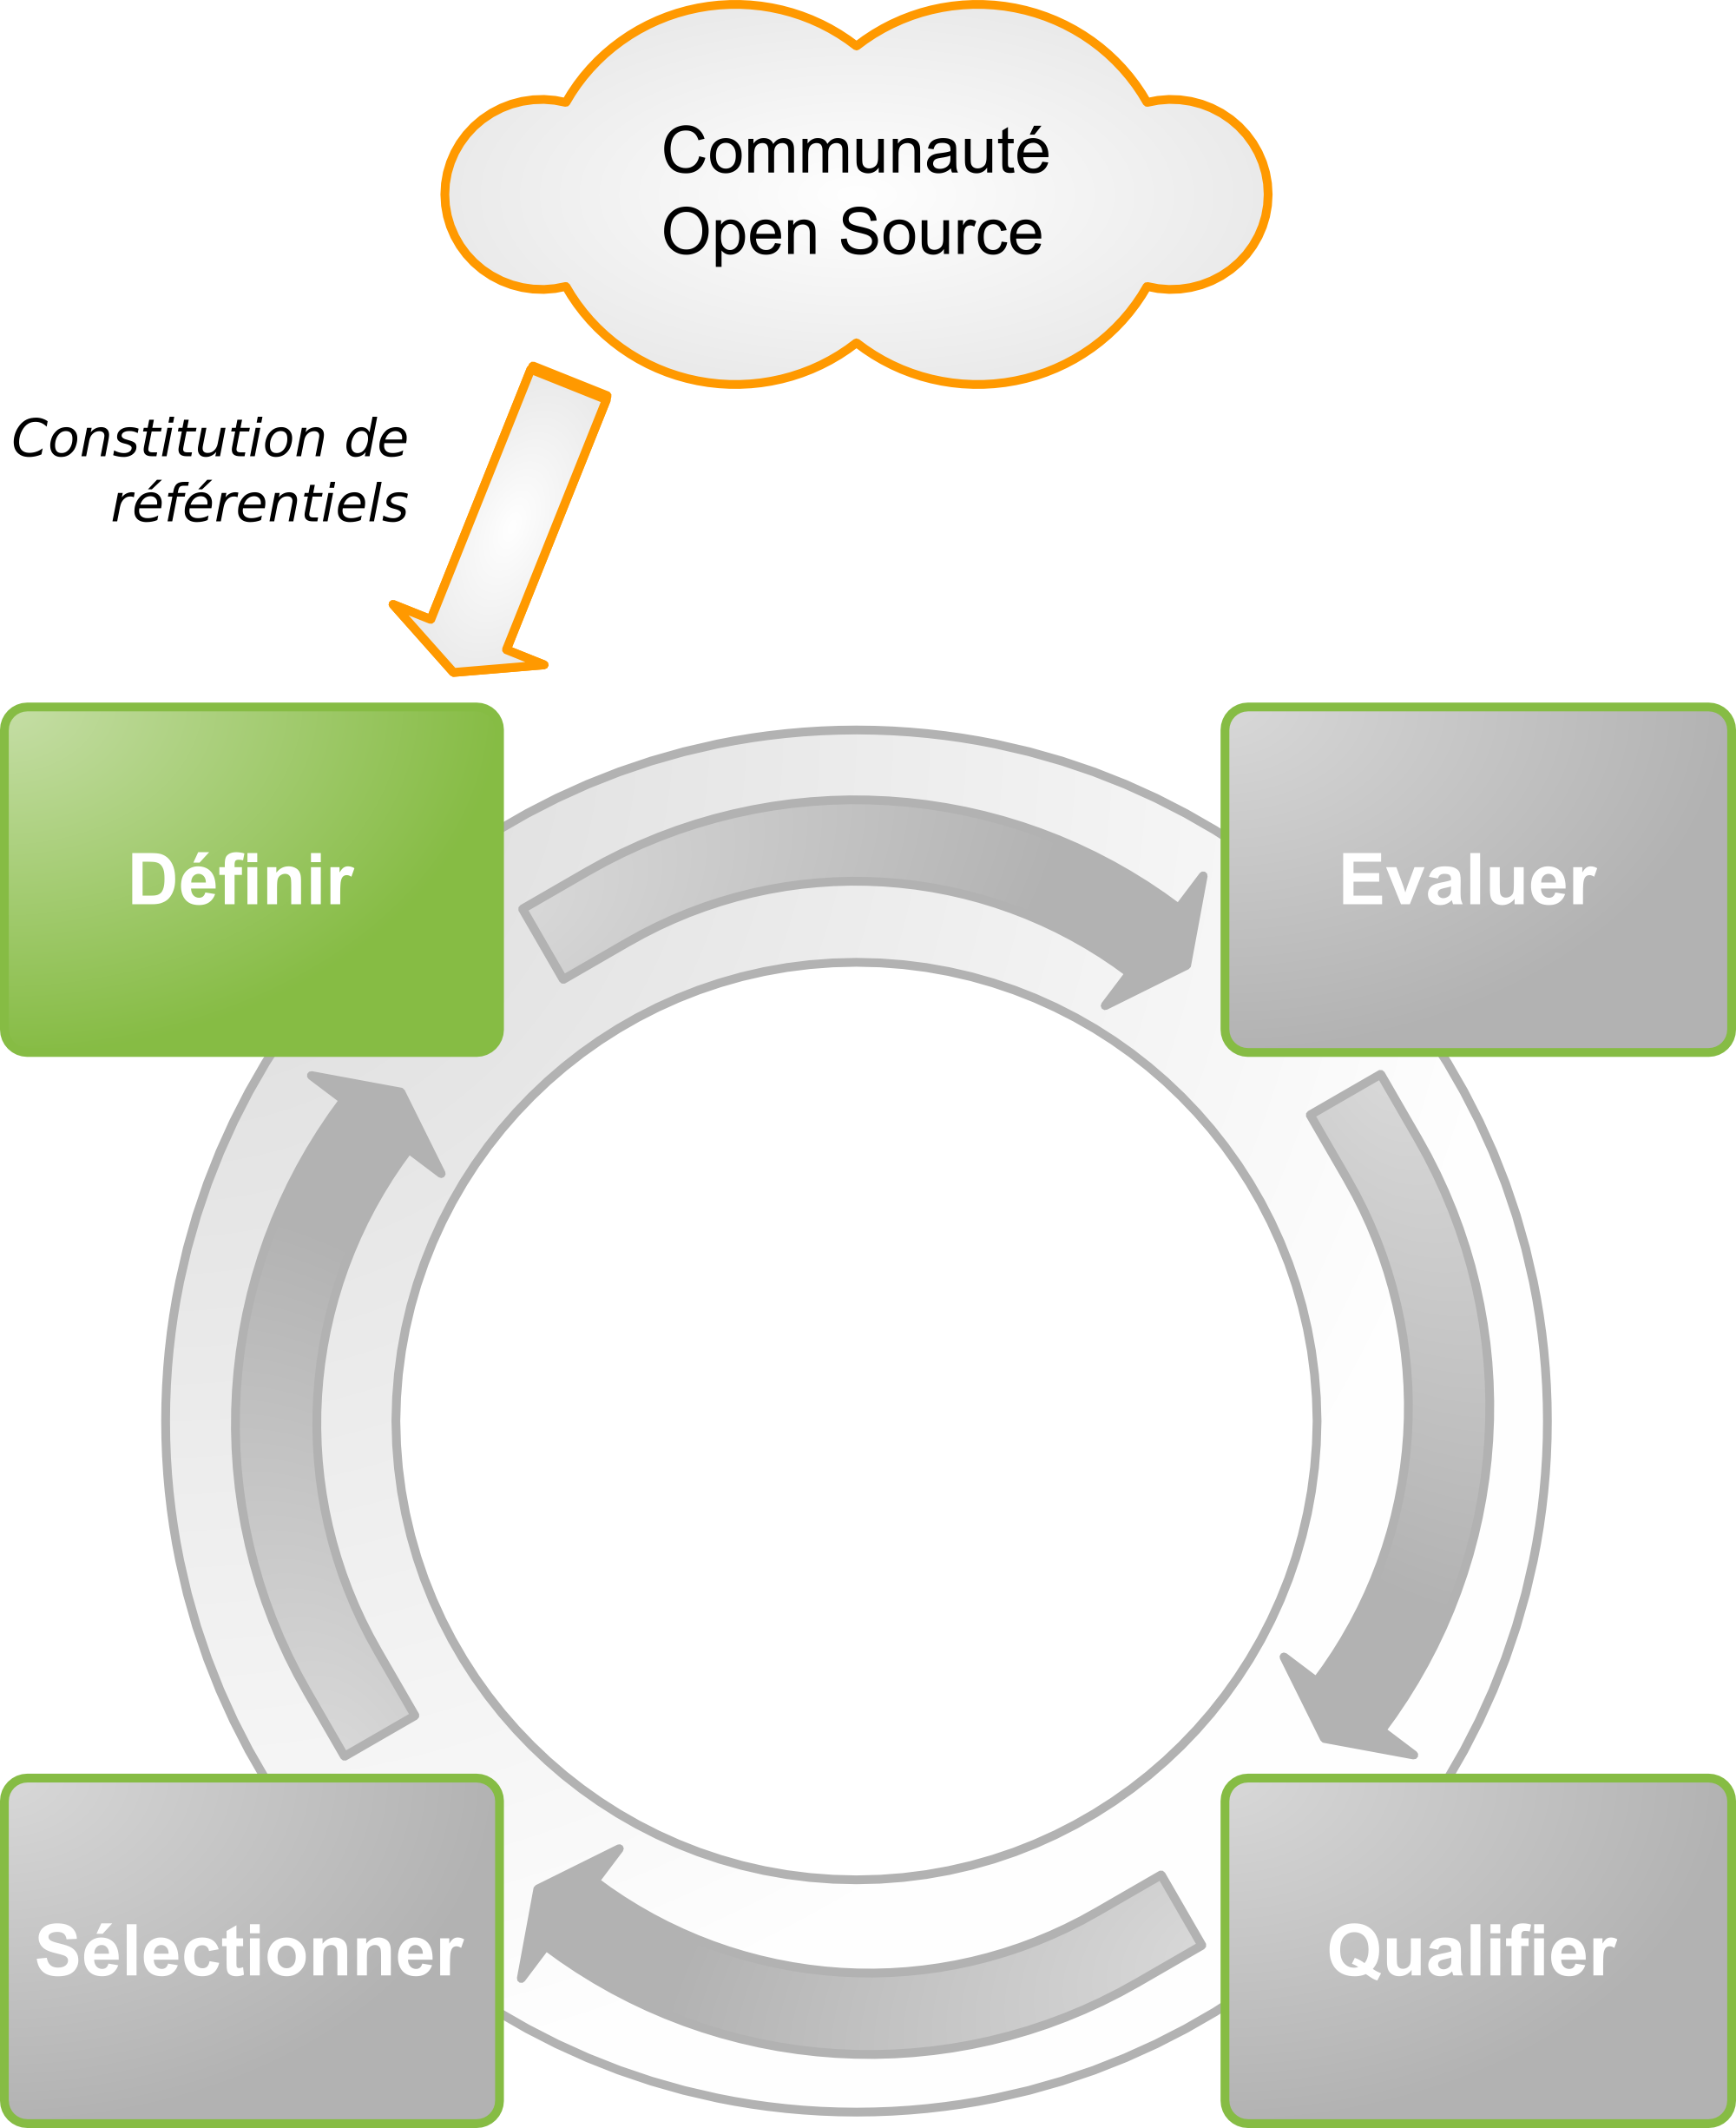
\includegraphics[width=10cm]{images/definir}
\caption{Step 1 - Define}
\end{figure}


\subsection{Objective}
The objective of this step is to define various elements of typology re-used by the three 
remaining steps of the general process.


The frames of reference concerned are :
\begin{description}
\item [Software families:] hierarchic classification of of software domains and description of functional grids associated to each domain.
\item [Types of licences:] classification of free and open source licenses.
\item [Types of communities:] classification of community organizations existing around a free or open source software and in charge of its life-cycle.
\end{description}


\subsection{Software families}
This frame of reference evolves the most because as a software evolves, it
offers new functionalities to be added to the frame of reference.

\subsection{Types of licences}
This frame of reference lists and classifies the major licences used for free and open source software.
The criteria chosen to describe such a license are:

\begin{description}
\item [Ownership:] can the derived code become proprietary or must it remain free?
\item [Virality:] is another module linked to the source code inevitably affected by the same license?
\item [Inheritance:] does the derived code inherit inevitably from the license or is it possible to apply additional restrictions to it?
\end{description}

The table~\ref{license-list} lists the most common licences compared regarding criteria formulated above.


\begin{figure}
\center
\begin{tabular}{|c|c|c|c|}
\hline \TS{License} & \TS{Ownership} & \TS{Virality} & \TS{Inheritance}\\
\hline GPL & No & Yes & Yes\\
\hline CeCILL & No & Yes & Yes\\
%TODO revenir sur LGPL
\hline LGPL & No & Partial & Yes\\
\hline BSD & Yes & No & No\\
\hline Artistic & Yes & No & No\\
\hline MIT & Yes & No & No\\
\hline Apache v1.1 & Yes & No & No\\
\hline Apache v2.0 & Yes & No & No\\
\hline MPL v1.1 & No & No & Yes\\
\hline Common Public License v1.1 & No & No & No\\
\hline Academic Free License v2.1 & Yes & No & No\\
\hline PHP License v3.0 & Yes & No & No\\
\hline Open Software License v2.0 & No & No & No\\
\hline Zope Public License v2.0 & Yes & No & No\\
%TODO idem
\hline Python SF License v2.0 & Yes & No & No\\
\hline
\end{tabular}
\caption{Non comprehensive list of licenses}
\label{license-list}
\end{figure}
Note that a single software can published under the terms of several licences (including closed source).

\subsection{Types of communities}
The types of communities identified to date are:
\begin{description}
\item [Insulated developer:] the software is developed and managed by only one person.
\item [Group of developers:] several persons collaborating in an informal or not industrialized way.
\item [Organization of developers:] group of developers managing the software life-cycle in a formalized way, generally based on role attribution (developer, tester, delivery manager...) and meritocracy.
\item [Legal Entity:] a legal entity (in general non lucrative) which manages the community, generally possesses copyrights and also manages sponsorship and linked subsidies.
\item [Commercial entity:] commercial organization employing the project's main developers who are remunerated by sale of services or of commercial versions of the software.
\end{description}


\subsection{O3S tool}
The O3S tool is designed to be able to easily manage these frames of reference and to measure 
impacts generated by modifications on data already collected during others QSOS steps.

%Copyright (c) 2004 2005 2006 Atos Origin
%Permission is granted to copy, distribute and/or modify this
%document
%under the terms of the GNU Free Documentation License,
%      Version 1.2
%      or any later version published by the Free Software
%      Foundation;
%      with no Invariant Sections, no Front-Cover
%      Texts, and no Back-Cover
%      Texts.  A copy of the license is
%      included in the section entitled "GNU
%      Free Documentation License".
%
%$Id: eval.tex,v 1.1 2006/02/16 16:33:33 goneri Exp $
\section{Evaluate}
\begin{figure}
\center
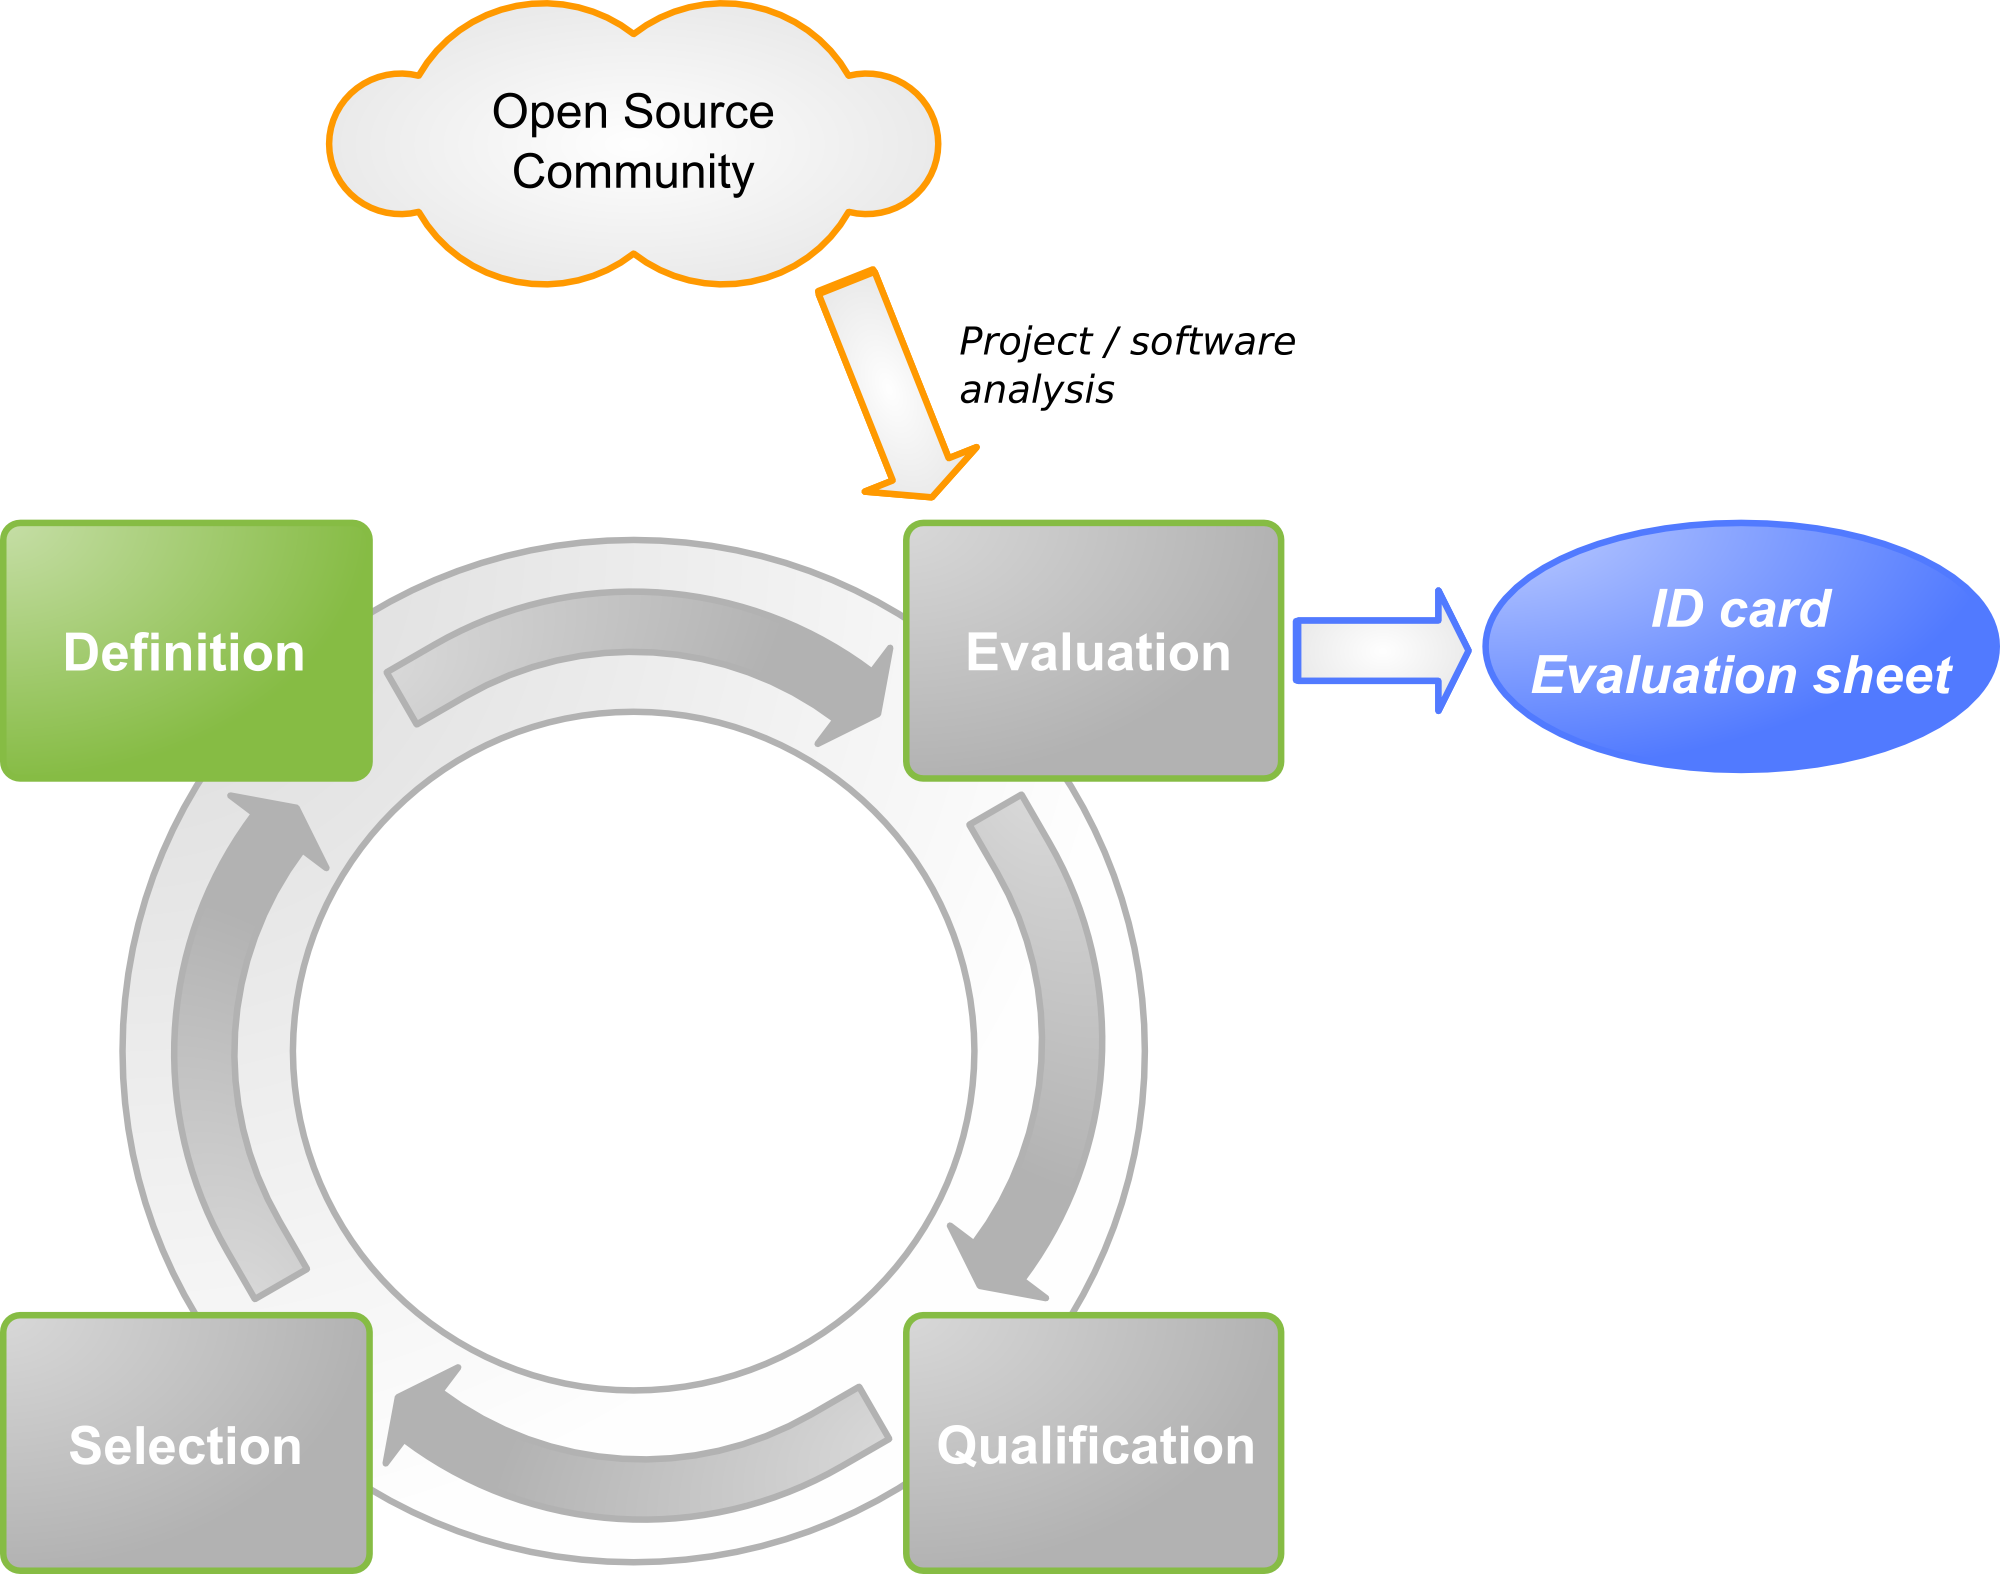
\includegraphics[width=13cm]{images/evaluer}
\caption{Step 2 - Evaluate}
\end{figure}


\subsection{Objective}
The objective of this step is to carry out the evaluation of the software. It consists in collecting information from the open source community, in order to:

\begin{itemize}
\item Build the identity card of a softwarev
\item Build the evaluation sheet of a software, by scoring tcriteria split on three major axis:
  \begin{itemize}
  \item Functional coverage
  \item Risks from user's perspective
  \item Risks from service provider's perspective
  \end{itemize}
\end{itemize}

This evaluation effort can be inserted in a more global approach of technological survey which is not completely described in this document.

\subsection{Identity card}
Data constituting the identity card is raw and factual and is not directly scored. Howerver it is used as a basis for the scoring process described below.


The main parts of an identity card are:


\subsubsection{General information}
\begin{itemize}
\item Name of the software
\item Reference, date of creation, date of release of the ID card
\item Author 
\item Type of software 
\item Brief description of the software
\item Licenses to which the software is subjected
\item Project's URI and demonstration site
\item Compatible operating systems
\item Fork's origin (if the software is a fork)
\end{itemize}

\subsubsection{Existing services}
\begin{itemize}
\item Documentation
\item Number of contractual support offers
\item Number of training offers
\item Number of consultancy offers
\end{itemize}

\subsubsection{Functional and technical aspects}
\begin{itemize}
\item Technologies of implementation
\item Technical prerequisites
\item Detailed functionalities
\item Roadmap
\end{itemize}

\subsubsection{Synthesis}
\begin{itemize}
\item General trend
\item Comments
\end{itemize}

%Copyright (c) 2004 2005 2006 Atos Origin
%Permission is granted to copy, distribute and/or modify this
%document
%under the terms of the GNU Free Documentation License,
%      Version 1.2
%      or any later version published by the Free Software
%      Foundation;
%      with no Invariant Sections, no Front-Cover
%      Texts, and no Back-Cover
%      Texts.  A copy of the license is
%      included in the section entitled "GNU
%      Free Documentation License".
%
%$Id: eval_app.tex,v 1.3 2006/03/31 12:08:12 goneri Exp $
\subsection{Evaluation sheet}
Every software release is described in an evaluation sheet. This document includes more detailed information 
than the identity card as it focuses on identifying, describing and analyzing in detail each 
evolution brought by the new release.
\subsubsection{Scoring}
Criteria are scored from 0 to 2. These scores will be used in Step 4 - "Selection" 
to compare and select software according to the weightings, representing the user's requirements 
specified in Step 3 - "Qualifcation".

The following paragraphs describe the criteria used for each axis of evaluation.
Note that the same criterion or similar criteria can appear on different axis.

\subsubsection{Functional coverage}
The functional grid is determined by the software's family and proceeds from the frame 
of reference of Step 1 - "Definition".
Consult the site \url{http://www.qsos.org} for details of functional grids by software families.

For each element of the grid, the scoring rule is as follows:


\begin{figure}
\center
\begin{tabular}{|c|c|c|}
\hline \TS{Functionality} & \TS{Score}\\
\hline Not covered & 0\\
\hline Partially covered & 1\\
\hline Completely covered & 2\\
\hline
\end{tabular}
\end{figure}


In certain cases it is necessary to use several functional grids for a same software, 
for instance when it belongs to more than one software family. 
In this case, the functional criteria are distributed on separated axis in order to be 
able to distinctly evaluate the functional coverage for each family.



\subsubsection{Risks from the user's perspective}

This axis of evaluation includes criteria to estimate risks incurred by the user when adopting 
free or open soure software.
Scoring of criteria is done independently of any particular user's context 
(the context is considered later in Step 3 - "Qualification").


Criteria are split into five categories:
\begin{itemize}
\item Intrinsic durability
\item Industrialized solution
\item Integration
\item Technical adaptability
\item Strategy
\end{itemize}


The following tables detail each one of these categories, by specifying the rule of notation 
to be used for each criterion.

%%%%%%%%%%%%%%%%%%%%%% Start Intrinsic durability
%%% Start Maturity
\begin{figure}
\center
\begin{tabular}{|p{2cm}|p{2cm}|p{2.8cm}|p{2.8cm}|p{2.8cm}|}
\hline \multicolumn{2}{|c|}{\TS{Intrinsic durability}} &
\multicolumn{3}{|c|}{\TS{Score}}\\
\cline{3-5} \multicolumn{2}{|c|}{} & \multicolumn{1}{|c|}{\TS{0}} &
\multicolumn{1}{|c|}{\TS{1}} &\multicolumn{1}{|c|}{\TS{2}}\\
\hline
\TS{Maturity}&
\TS{Age}&
For instance less than 3 months&
For instance between 3 months and 3 years &
For instance more than 3 years \\
\cline{2-5}&
\TS{Stability}&
Unstable software with numerous releases or patches generating side effects&
Stabilized production release existing but old. Difficulties to stabilize development releases&
Stabilized software. Releases provide bug fixes corrections but mainly new functionalities \\
\cline{2-5}&
\TS{History, known problems}&
Software knows several problems which can be prohibitive&
No known major problem or crisis&
History of good management of crisis situations\\
\cline{2-5}&
\TS{Fork probability, source of Forking}&
Software is very likely to be forked in the future&
Software comes from a fork but has very few chances of being forked in the future&
Software has very little chance of being forked. It does not come from a fork either\\
\hline
\end{tabular}
\end{figure}
%%% End Maturity

%%% Start Adoption 
\begin{figure}
\center
\begin{tabular}{|p{2cm}|p{2cm}|p{2.8cm}|p{2.8cm}|p{2.8cm}|}
\hline \multicolumn{2}{|c|}{\TS{Intrinsic durability}} &
\multicolumn{3}{|c|}{\TS{Score}}\\
\cline{3-5} \multicolumn{2}{|c|}{} & \multicolumn{1}{|c|}{\TS{0}} &
\multicolumn{1}{|c|}{\TS{1}} &\multicolumn{1}{|c|}{\TS{2}}\\
\hline
\TS{Adoption}&
\TS{Popularity (related to: general public, niche, ...)}&
Very few users identified&
Detectable use on Internet (sourceforge, freshmeat, google, ...)&
Numerous users, numerous references\\
\cline{2-5}&
\TS{References}&
None&
Few references, non critical usages&
Often implemented for critical applications\\
\cline{2-5}&
\TS{Contributing community}&
No community or without real activity (forum, mailing list,...)&
Existing community with a notable activity&
Strong community: big activity on forums, numerous contributors and advocates\\
\cline{2-5}&
\TS{Books}&
No book about the software&
Less than 5 books about the software are available&
More than 5 books about software are available, in several languages\\
\hline
\end{tabular}
\end{figure}
%%% End Adoption 

%%% Start Development leadership
\begin{figure}
\center
\begin{tabular}{|p{2cm}|p{2cm}|p{2.8cm}|p{2.8cm}|p{2.8cm}|}
\hline \multicolumn{2}{|c|}{\TS{Intrinsic durability}} &
\multicolumn{3}{|c|}{\TS{Score}}\\
\cline{3-5} \multicolumn{2}{|c|}{} & \multicolumn{1}{|c|}{\TS{0}} &
\multicolumn{1}{|c|}{\TS{1}} &\multicolumn{1}{|c|}{\TS{2}}\\
\hline
\TS{Development leadership}&
\TS{Leading team}&
1 to 2 individuals involved, not clearly identified&
Between 2 and 5 independent people&
More than 5 people\\
\cline{2-5}&
\TS{Management style}&
Complete dictatorship&
Enlightened despotism&
Council of architects with identified leader (e.g: ASF, ...)\\
\hline
\end{tabular}
\end{figure}
%%% End Development leadership

%%% Start Activity
\begin{figure}
\center
\begin{tabular}{|p{2cm}|p{2cm}|p{2.8cm}|p{2.8cm}|p{2.8cm}|}
\hline \multicolumn{2}{|c|}{\TS{Intrinsic durability}} &
\multicolumn{3}{|c|}{\TS{Score}}\\
\cline{3-5} \multicolumn{2}{|c|}{} & \multicolumn{1}{|c|}{\TS{0}} &
\multicolumn{1}{|c|}{\TS{1}} &\multicolumn{1}{|c|}{\TS{2}}\\
\hline
\TS{Activity}&
\TS{Developers, identification, turnover}&
Less than 3 developers, not clearly identified&
Between 4 and 7 developers, or more unidentified developers with important turnover&
More than 7 developers clearly identified, very stable team\\
\cline{2-5}&
\TS{Activity on bugs}&
Slow reactivity in forum or on mailing list, or nothing regarding bug fixes in release notes&
Detectable activity but without process clearly exposed, long reaction/resolution time&
Strong reactivity based on roles and tasks assignment\\

\cline{2-5}&
\TS{Activity on functionalities}&
No or few new functionalities&
Evolution of the product driven by the core team or by user's request without any clearly explained process&
Tool(s) to manage feature requests, strong interaction with roadmap\\
\cline{2-5}&
\TS{Activity on releases}&
Very weak activity on both production and development releases&
Activity on production and development releases. Frequent minor releases (bug fixes)&
Important activity with frequent minor releases (bugs fixes) and planned major 
releases relating to the roadmap forcast\\
\hline
\end{tabular}
\end{figure}
%%% End Activity


%%% Start Independence of developments 
\begin{figure}
\center
\begin{tabular}{|p{2cm}|p{2cm}|p{2.8cm}|p{2.8cm}|p{2.8cm}|}
\hline \multicolumn{2}{|c|}{\TS{Intrinsic durability}} &
\multicolumn{3}{|c|}{\TS{Score}}\\
\cline{3-5} \multicolumn{2}{|c|}{} & \multicolumn{1}{|c|}{\TS{0}} &
\multicolumn{1}{|c|}{\TS{1}} &\multicolumn{1}{|c|}{\TS{2}}\\
\hline
\TS{Independence of developments}&
\TS{Independence of developments}&
Developments realized at 100\% by employees of a single company&
60\% maximum&
20\% maximum\\
\hline
\end{tabular}
\end{figure}
%%% End Independence of developments

% Le clearpage impose a Latex de poser les objets flotant qu'il a en memoire
% ! LaTeX Error: Too many unprocessed floats.
% TODO : le must serait de ne pas utiliser de float
\clearpage
%%%%%%%%%%%%%%%%%%%%%% End Intrinsic durability

%%%%%%%%%%%%%%%%%%%%%% Start Industrialised solution
%%% Start Services 
\begin{figure}
\center
\begin{tabular}{|p{2cm}|p{2cm}|p{2.8cm}|p{2.8cm}|p{2.8cm}|}
\hline \multicolumn{2}{|c|}{\TS{Industrialised solution}} &
\multicolumn{3}{|c|}{\TS{Score}}\\
\cline{3-5} \multicolumn{2}{|c|}{} & \multicolumn{1}{|c|}{\TS{0}} &
\multicolumn{1}{|c|}{\TS{1}} &\multicolumn{1}{|c|}{\TS{2}}\\
\hline
\TS{Services}&
\TS{Training}&
No offer of training identified&
Offer exists but is restricted geographically and to one language or is provided by a single contractor&
Rich offers provided by several contractors, in several languages and split into modules of gradual levels\\
\cline{2-5}&
\TS{Support}&
No offer of support except via public forums and mailing lists&
Offer exists but is provided by a single contractor without strong commitment quality of services&
Multiple service providers with strong commitment (e.g: guaranteed resolution time)\\
\cline{2-5}&
\TS{Consulting}&
No offer of consulting service&
Offer exists but is restricted geographically and to one language or is provided by a single contractor&
Consulting services provided by different contractors in several languages\\
\hline
\end{tabular}
\end{figure}
%%% End Services 

%%% Start Documentation 
\begin{figure}
\center
\begin{tabular}{|p{2cm}|p{2cm}|p{2.8cm}|p{2.8cm}|p{2.8cm}|}
\hline \multicolumn{2}{|c|}{\TS{Industrialised solution}} &
\multicolumn{3}{|c|}\TS{{Score}}\\
\cline{3-5} \multicolumn{2}{|c|}{} & \multicolumn{1}{|c|}{\TS{0}} &
\multicolumn{1}{|c|}{\TS{1}} &\multicolumn{1}{|c|}{\TS{2}}\\
\hline
\TS{Documenta\-tion}&
\TS{Documenta\-tion}&
No user documentation&
Documentation exists but shifted in time, is restricted to one language or is poorly detailed&
Documentation always up to date, translated and possibly adapted to different target readers 
(end user, sysadmin, manager, ?)\\
\hline
\end{tabular}
\end{figure}
%%% End Documentation 

%%% Start Quality Assurance
\begin{figure}
\center
\begin{tabular}{|p{2cm}|p{2cm}|p{2.8cm}|p{2.8cm}|p{2.8cm}|}
\hline \multicolumn{2}{|c|}{\TS{Industrialised solution}} &
\multicolumn{3}{|c|}{\TS{Score}}\\
\cline{3-5} \multicolumn{2}{|c|}{} & \multicolumn{1}{|c|}{\TS{0}} &
\multicolumn{1}{|c|}{\TS{1}} &\multicolumn{1}{|c|}{\TS{2}}\\
\hline
\TS{Quality Assurance}&
\TS{Quality Assurance}&
No QA process&
Identifies QA process but not much formalized and with no tool&
Automatic testing process included in code's life-cycle with publication of results\\
\cline{2-5}&
\TS{Tools}&
No bug or feature request management tool&
Standard tools provided (for instance by a hosting forge) but poorly used&
Very active use of tools for roles/tasks allocation and progess monitoring\\
\hline
\end{tabular}
\end{figure}
%%% End Quality Assurance 

%%% Start Exploitability
\begin{figure}
\center
\begin{tabular}{|p{2cm}|p{2cm}|p{2.8cm}|p{2.8cm}|p{2.8cm}|}
\hline \multicolumn{2}{|c|}{\TS{Industrialised solution}} &
\multicolumn{3}{|c|}{\TS{Score}}\\
\cline{3-5} \multicolumn{2}{|c|}{} & \multicolumn{1}{|c|}{\TS{0}} &
\multicolumn{1}{|c|}{\TS{1}} &\multicolumn{1}{|c|}{\TS{2}}\\
\hline
\TS{Exploitability}&
\TS{Installation, deployment}&
Complicated installation without any tools and no global deployment management&
Easy installation (e.g: file copy/unzip) but without global deployment management&
Very simple installation and/or existence of evolved tools: installers, global deployment console, ...\\
\cline{2-5}&
\TS{Ease of use, ergonomics}&
Difficult to use, requires an in depth knowledge of the software functionality&
Austere and very technical ergonomics&
GUI including help functions and elaborated ergonomics (e.g: skins/themes management)\\
\cline{2-5}&
\TS{Administration / Monitoring}&
No administrative or monitoring functionalities&
Existing functionalities but incomplete and in need of improvement&
Complete and easy-to-use administration and monitoring functionalities. Possible integration with 
external tools (e.g: via SNMP, ...)\\
\hline
\end{tabular}
\end{figure}
%%% End Exploitability
%%%%%%%%%%%%%%%%%%%%%% End Industrialised solution

%%%%%%%%%%%%%%%%%%%%%% Start Integration 
%%% Start Adherence to standards
\begin{figure}
\center
\begin{tabular}{|p{2cm}|p{2cm}|p{2.8cm}|p{2.8cm}|p{2.8cm}|}
\hline \multicolumn{2}{|c|}{\TS{Integration}} & \multicolumn{3}{|c|}{\TS{Score}}\\
\cline{3-5} \multicolumn{2}{|c|}{} & \multicolumn{1}{|c|}{\TS{0}} &
\multicolumn{1}{|c|}{\TS{1}} &\multicolumn{1}{|c|}{\TS{2}}\\
\hline
\TS{Adherence to standards}&
\TS{Adherence to standards}&
Software uses its own implementations that do not conform to official or 'de facto' standards&
Adherence to standards on certain functionalities allowing to interface with other software&
The notion of interfacing standards is clearly a choice of design and it is very easy to integrate it with other software\\
\hline
\end{tabular}
\end{figure}
%%% End Adherence to standards

%%% Start Interface with other products
\begin{figure}
\center
\begin{tabular}{|p{2cm}|p{2cm}|p{2.8cm}|p{2.8cm}|p{2.8cm}|}
\hline \multicolumn{2}{|c|}{\TS{Integration}} & \multicolumn{3}{|c|}{\TS{Score}}\\
\cline{3-5} \multicolumn{2}{|c|}{} & \multicolumn{1}{|c|}{\TS{0}} &
\multicolumn{1}{|c|}{\TS{1}} &\multicolumn{1}{|c|}{\TS{2}}\\
\hline
\TS{Interface with other products}&
\TS{Interface with other products (independently of adherence to standards)}&
Software communicates with no other software&
Existence of interfaces or conversion to or from third party software&
Numerous possibilities of integration with third party software\\
\hline
\end{tabular}
\end{figure}
%%% End Interface with other products
%%%%%%%%%%%%%%%%%%%%%% End Integration

%%%%%%%%%%%%%%%%%%%%%% Start Technical adaptability
%%% Start Modularity
\begin{figure}
\center
\begin{tabular}{|p{2cm}|p{2cm}|p{2.8cm}|p{2.8cm}|p{2.8cm}|}
\hline \multicolumn{2}{|c|}{\TS{Technical adaptability}} &
\multicolumn{3}{|c|}{\TS{Score}}\\
\cline{3-5} \multicolumn{2}{|c|}{} & \multicolumn{1}{|c|}{\TS{0}} &
\multicolumn{1}{|c|}{\TS{1}} &\multicolumn{1}{|c|}{\TS{2}}\\
\hline
\TS{Modularity}&
\TS{Modularity}&
Monolithic software&
Presence of high level modules allowing a first level of software adaptation&
Modular conception, allowing easy adaptation of the software by selecting modules or even developing new ones\\
\hline
\end{tabular}
\end{figure}
%%% End Modularity

%%% Start By-products
\begin{figure}
\center
\begin{tabular}{|p{2cm}|p{2cm}|p{2.8cm}|p{2.8cm}|p{2.8cm}|}
\hline \multicolumn{2}{|c|}{\TS{Technical adaptability}} &
\multicolumn{3}{|c|}{\TS{Score}}\\
\cline{3-5} \multicolumn{2}{|c|}{} & \multicolumn{1}{|c|}{\TS{0}} &
\multicolumn{1}{|c|}{\TS{1}} &\multicolumn{1}{|c|}{\TS{2}}\\
\hline
\TS{By-products}&
\TS{Code modification}&
Everything by hand&
Recompilation possible but complex without any tools or documentation&
Recompilation with tools (e.g: make, ANT, ...) and documention provided\\
\cline{2-5}&
\TS{Code extension}&
Any modification requires code recompilation&
Architecture designed for static extension but requires recompilation&
Principle of plug-in, architecture designed for dynamic extension without recompilation\\
\hline
\end{tabular}
\end{figure}
%%% End By-products
%%%%%%%%%%%%%%%%%%%%%% End Technical adaptability

%%%%%%%%%%%%%%%%%%%%%% Start Strategy 
%%% Start License 
\begin{figure}
\center
\begin{tabular}{|p{2cm}|p{2cm}|p{2.8cm}|p{2.8cm}|p{2.8cm}|}
\hline \multicolumn{2}{|c|}{\TS{Strategy}} & \multicolumn{3}{|c|}{\TS{Score}}\\
\cline{3-5} \multicolumn{2}{|c|}{} & \multicolumn{1}{|c|}{\TS{0}} &
\multicolumn{1}{|c|}{\TS{1}} &\multicolumn{1}{|c|}{\TS{2}}\\
\hline
\TS{License}&
\TS{Permissiveness (to be weighted only if user wants to become owner of code)}&
Very strict license, like GPL&
Moderate permissive license located between both extremes (GPL and BSD), dual-licensing depending on 
the type of user (person, company, ...) or their activities&
Very permissive like BSD or Apache licenses\\
\cline{2-5}&
\TS{Protection against proprietary forks}&
Very permissive like BSD or Apache licenses&
Moderate permissive license located between both extremes (GPL and BSD), dual-licensing depending on 
the type of user (person, company, ...) or their activities&
Very strict license, like GPL\\
\hline
\end{tabular}
\end{figure}
%%% End License 

%%% Start Copyright owners
\begin{figure}
\center
\begin{tabular}{|p{2cm}|p{2cm}|p{2.8cm}|p{2.8cm}|p{2.8cm}|}
\hline \multicolumn{2}{|c|}{\TS{Strategy}} & \multicolumn{3}{|c|}{\TS{Score}}\\
\cline{3-5} \multicolumn{2}{|c|}{} & \multicolumn{1}{|c|}{\TS{0}} &
\multicolumn{1}{|c|}{\TS{1}} &\multicolumn{1}{|c|}{\TS{2}}\\
\hline
\TS{Copyright owners}&
\TS{Copyright owners}&
Rights held by a few individuals or entities, making it easier to change the license&
Rights held by numerous individuals owning the code in a homogeneous way, making relicensing very difficult&
Rights held by a legal entity in whom the community trusts (e.g. FSF or ASF)\\
\hline
\end{tabular}
\end{figure}
%%% End Copyright owners

%%% Start Modification of source code
\begin{figure}
\center
\begin{tabular}{|p{2cm}|p{2cm}|p{2.8cm}|p{2.8cm}|p{2.8cm}|}
\hline \multicolumn{2}{|c|}{\TS{Strategy}} & \multicolumn{3}{|c|}{\TS{Score}}\\
\cline{3-5} \multicolumn{2}{|c|}{} & \multicolumn{1}{|c|}{\TS{0}} &
\multicolumn{1}{|c|}{\TS{1}} &\multicolumn{1}{|c|}{\TS{2}}\\
\hline
\TS{Modification of source code}&
\TS{Modification of source code}&
No practical way to propose code modifications&
Tools provided to access and modify code (like CVS or SVN) but not really used to develop the software&
The code modification process is well defined, exposed and respected, based on roles assignment\\
\hline
\end{tabular}
\end{figure}
%%% End Modification of source code

%%% Start roadmap 
\begin{figure}
\center
\begin{tabular}{|p{2cm}|p{2cm}|p{2.8cm}|p{2.8cm}|p{2.8cm}|}
\hline \multicolumn{2}{|c|}{\TS{Strategy}} & \multicolumn{3}{|c|}{\TS{Score}}\\
\cline{3-5} \multicolumn{2}{|c|}{} & \multicolumn{1}{|c|}{\TS{0}} &
\multicolumn{1}{|c|}{\TS{1}} &\multicolumn{1}{|c|}{\TS{2}}\\
\hline
\TS{Roadmap}&
\TS{Roadmap}&
No published roadmap&
Existing roadmap without planning&
Versionned roadmap, with planning and measure of delays\\
\hline
\end{tabular}
\end{figure}
%%% End Roadmap

%%% Start Sponsor 
\begin{figure}
\center
\begin{tabular}{|p{2cm}|p{2cm}|p{2.8cm}|p{2.8cm}|p{2.8cm}|}
\hline \multicolumn{2}{|c|}{\TS{Strategy}} & \multicolumn{3}{|c|}{\TS{Score}}\\
\cline{3-5} \multicolumn{2}{|c|}{} & \multicolumn{1}{|c|}{\TS{0}} &
\multicolumn{1}{|c|}{\TS{1}} &\multicolumn{1}{|c|}{\TS{2}}\\
\hline
\TS{Sponsor}&
\TS{Sponsor}&
Software has no sponsor, the core team is not paid&
Software has an unique sponsor who might determine its strategy&
Software is sponsored by industry\\
\hline
\end{tabular}
\end{figure}
%%% Start Sponsor 

%%% Start Strategical independence
\begin{figure}
\center
\begin{tabular}{|p{2cm}|p{2cm}|p{2.8cm}|p{2.8cm}|p{2.8cm}|}
\hline \multicolumn{2}{|c|}{\TS{Strategy}} & \multicolumn{3}{|c|}{\TS{Score}}\\
\cline{3-5} \multicolumn{2}{|c|}{} & \multicolumn{1}{|c|}{\TS{0}} &
\multicolumn{1}{|c|}{\TS{1}} &\multicolumn{1}{|c|}{\TS{2}}\\
\hline
\TS{Strategical independence}&
\TS{Strategical independence}&
No detectable strategy or strong dependency on one unique actor (person, company, sponsor, ...)&
Strategical vision shared with several other free and open source projects but without strong 
commitment from copyrights owners&
Strong independence of the core team, legal entity holding rights, strong involvement in the standardization process\\
\hline
\end{tabular}
\end{figure}
%%% End Strategical independence
%%%%%%%%%%%%%%%%%%%%%% End Strategy 

\clearpage

\subsubsection{Risks from the service provider's perspective}
This axis of evaluation regroups criteria to estimate risks incurred by a contractor offering services around a free or open source software (expertise, intregration, development, support, ...). It is notably on this basis that its level of commitment can be determined.

%%%%%%%%%%%%%%%%%%%%%% Start Services provinding
%%% Start Maintenability
\begin{figure}
\center
\begin{tabular}{|p{2cm}|p{2cm}|p{2.8cm}|p{2.8cm}|p{2.8cm}|}
\hline \multicolumn{2}{|c|}{\TS{Services provinding}} & \multicolumn{3}{|c|}{\TS{Score}}\\
\cline{3-5} \multicolumn{2}{|c|}{} & \multicolumn{1}{|c|}{\TS{0}} &
\multicolumn{1}{|c|}{\TS{1}} &\multicolumn{1}{|c|}{\TS{2}}\\
\hline
\TS{Maintenability}&
\TS{Quality of source code}&
Not very readable code or of poor quality, incoherence in coding styles&
Readable code but not really commented in detail&
Readable and commented code, implementing classic design patterns with a coherent and applied coding policy\\
\cline{2-5}&
\TS{Technological dispersion}&
Use of numerous different languages&
One main language with certain modules coded in other languages for specific and limited requirements&
One unique language\\
\cline{2-5}&
\TS{Intrinsic complexity}&
Very complex code requiring high level of expertise to perform modifications without generating side effects&
Not very complex code but still requiring expertise in programming languages and software design&
Simple code and design, easy to modify\\
\cline{2-5}&
\TS{Technical documentation}&
No documentation (development guide or automatically generated doc like javadoc)&
Incomplete or old documentation without conception and architectural considerations&
Detailed and up to date documentation, including conception, architecture design and coding considerations\\
\hline
\end{tabular}
\end{figure}
%%% Start Maintenability

%%% Start Code mastery
\begin{figure}
\center
\begin{tabular}{|p{2cm}|p{2cm}|p{2.8cm}|p{2.8cm}|p{2.8cm}|}
\hline \multicolumn{2}{|c|}{\TS{Services provinding}} & \multicolumn{3}{|c|}{\TS{Score}}\\
\cline{3-5} \multicolumn{2}{|c|}{} & \multicolumn{1}{|c|}{\TS{0}} &
\multicolumn{1}{|c|}{\TS{1}} &\multicolumn{1}{|c|}{\TS{2}}\\
\hline
\TS{Code mastery}&
\TS{Direct}&
No direct expertise of the source code&
Mastery of code but limited to a single person or to only a part of the source&
Several individuals mastering the code and covering together the totality of the source\\
\cline{2-5}&
\TS{Indirect}&
No indirect expertise on the source code&
Strong mastery via external expertise provided by partners&
Partnership with the copyrights owner and/or the core team\\
\hline
\end{tabular}
\end{figure}
%%% End Code mastery
%%%%%%%%%%%%%%%%%%%%%% End Services provinding
\clearpage


\subsubsection{Granularity of scores}
As stated above, it is possible to iterate the QSOS process. 
At the evaluation step this brings the capacity to score criteria in 
three passes with different levels of granularity:

\begin{itemize}
\item First the five main categories
\item Then the sub categories of each category
\item Finally every remaining criterion
\end{itemize}


The general process is thus not hindered if not all of the scored criteria are available.


Once all criteria have been scored, the score of the firsts two levels is calculated by the weighed average of scores of the direcly inferior level.

\subsection{O3S tool}
The O3S tool allows the entry of raw data and the evaluation of software on the three majors axis, 
as well as generation of the identidy cards of evaluated software.


The granularity of evaluation is managed as follows: as long as all
criteria composing a sub category are not scored, its score is not 
calculated but entered by the user. As soon as all criteria are scored, 
its score is then automatically calculated.

%Copyright (c) 2004 2005 2006 Atos Origin
%Permission is granted to copy, distribute and/or modify this
%document
%under the terms of the GNU Free Documentation License,
%      Version 1.2
%      or any later version published by the Free Software
%      Foundation;
%      with no Invariant Sections, no Front-Cover
%      Texts, and no Back-Cover
%      Texts.  A copy of the license is
%      included in the section entitled "GNU
%      Free Documentation License".
%
%$Id: qualify.tex,v 1.2 2006/03/07 16:35:51 rsemeteys Exp $
\section{Qualification}
\begin{figure}[h]
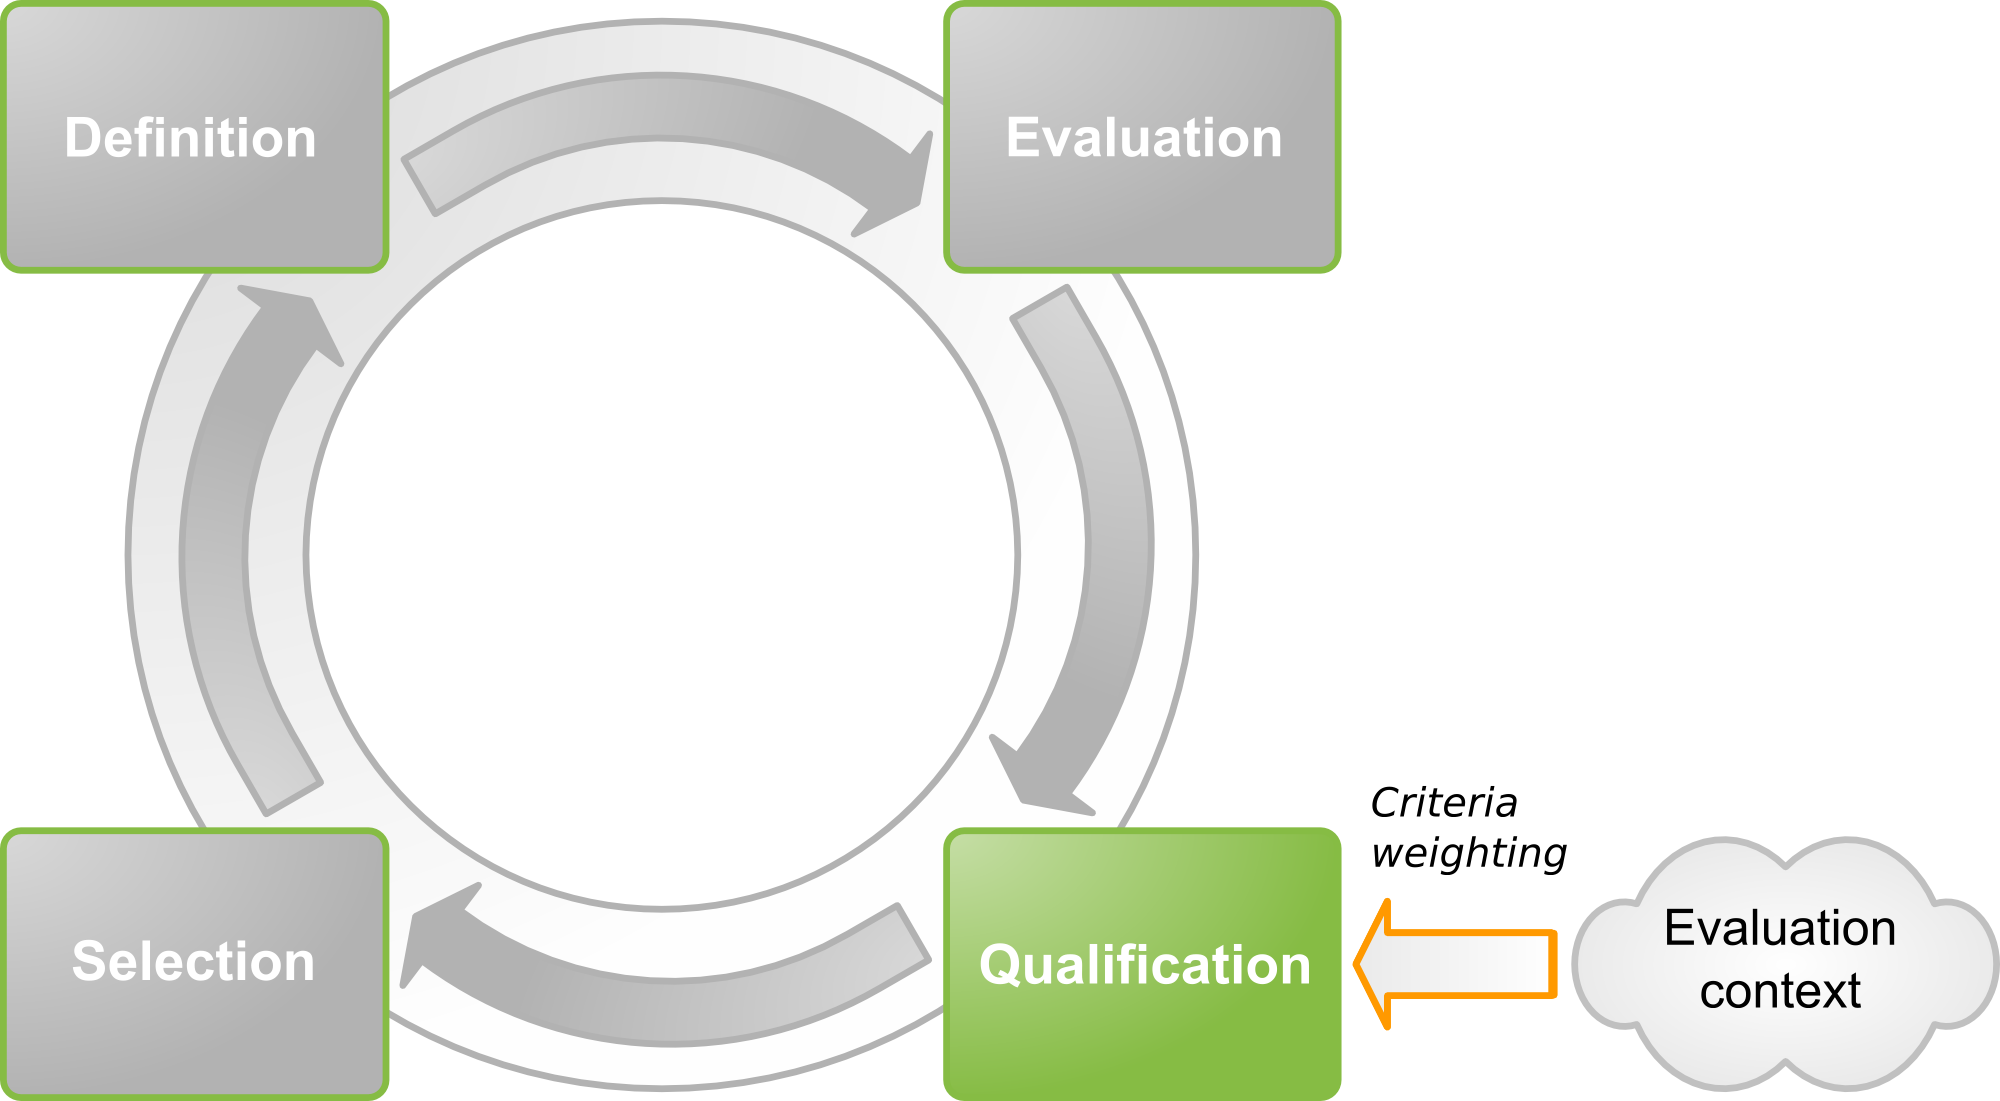
\includegraphics[width=13cm]{images/qualifier}
\caption{Step 3 - Qualification}
\end{figure}

\subsection{Objective}
The objective of this step is to define filters translating the needs and constraints 
related to the selection of free or open source software in a specific context. 
This is achieved by qualifying the user's context which will be used later in Step - 4 "Selection".


\subsection{Filter on ID card}
A first level of filtering can be defined on data from the software's ID card.


For instance, it could be to consider software only from a given family or 
software that's compatible with a given operating system.


In general, although it is not mandatory, this filter does not include 
any weighting; it is mostly used to eliminate inadequate software 
in the specific context of the user.

\subsection{Filter on Functional grid}
Each functionality of the functional grid is attributed a requirement 
level selected among the following:

\begin{itemize}
\item required functionality
\item optional functionality
\item not required functionality
\end{itemize}

These requirement levels will be linked to weighting values at Step 4 - "Selection", 
according to the selected mode of selection.

\subsection{Filter on User's risks}
The relevance of each criterion of this axis is positioned according to user's 
context, as indicated in figure~\ref{fig-relevance}.

\begin{figure}
\center
\begin{tabular}{|c|}
\hline \TS{Relevance}\\
\hline Irrelevant criterion, excluded from filter\\
\hline Relevant criterion\\
\hline Critical criterion\\
\hline
\end{tabular}
\label{fig-relevance}
\end{figure}
This relevance will be converted into a numerical weighting value at the following step, 
according to the chosen mode of selection.

\subsection {Filter on Service Provider's risks}
This filter is used by a service provider to evaluate software and services to be integrated into its offering and to determine the associated levels of commitment.


\subsection {O3S tool}
The O3S tool allows the definition of these different filters, while being guided with data entry.
%Copyright (c) 2004 2005 2006 Atos Origin
%Permission is granted to copy, distribute and/or modify this
%document
%under the terms of the GNU Free Documentation License,
%      Version 1.2
%      or any later version published by the Free Software
%      Foundation;
%      with no Invariant Sections, no Front-Cover
%      Texts, and no Back-Cover
%      Texts.  A copy of the license is
%      included in the section entitled "GNU
%      Free Documentation License".
%
%$Id: select.tex,v 1.2 2006/03/07 16:35:51 rsemeteys Exp $
\section{Selection}
\begin{figure}[h]
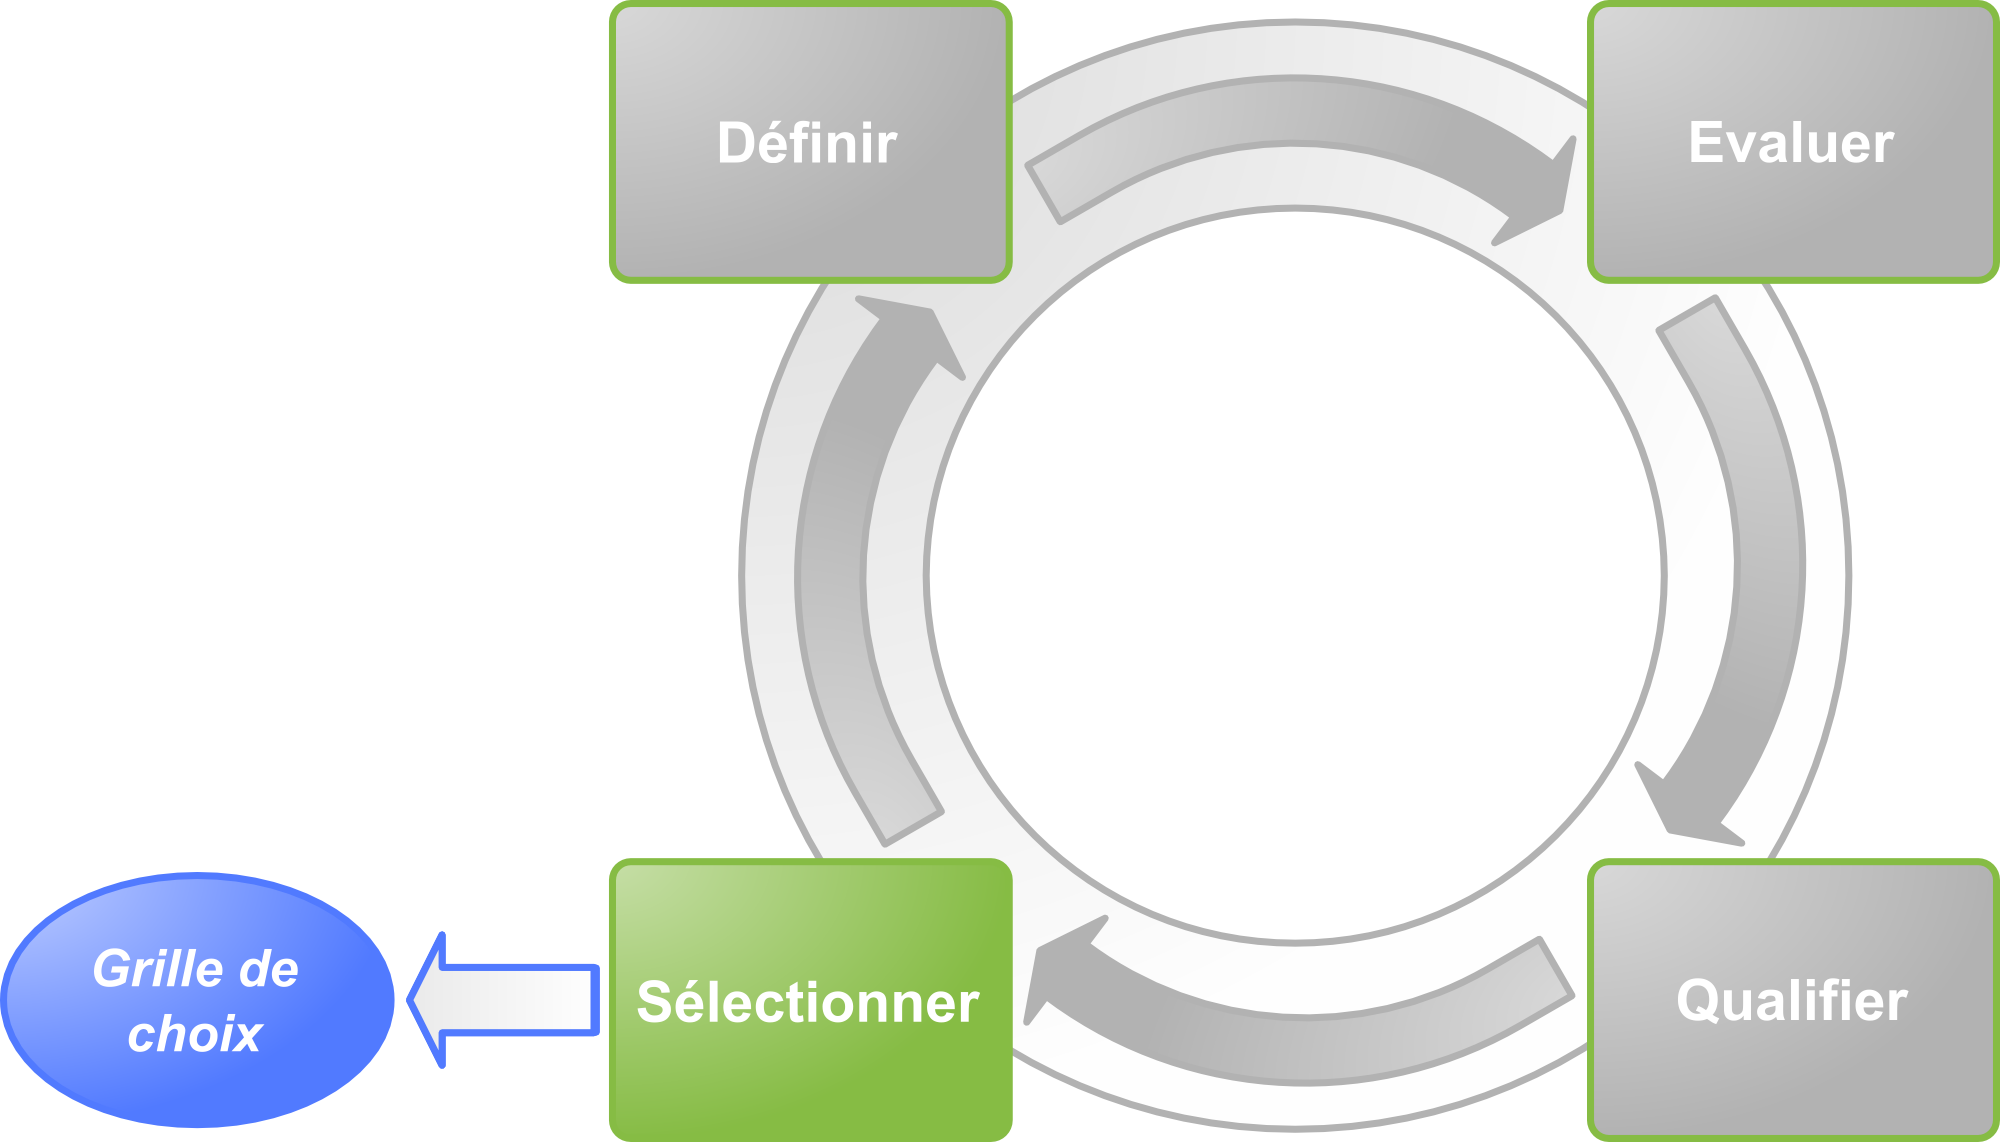
\includegraphics[width=13cm]{images/selectionner}
\caption{Step 4 - Selection}
\end{figure}

\subsection{Objective}
The objective of this step is to identify software fulfilling user's requirements, 
or more generally to compare software from the same family.

\subsection{Selection}
Two modes are possible:
\begin{itemize}
\item strict selection
\item loose selection
\end{itemize}


\subsubsection{Strict selection}
Strict selection is based on direct elimination as soon as software
does not fulfill the requirements formulated in Step 3 - "Qualification":

\begin{itemize}
\item Elimination of software incompatible with the filter on the ID card
\item Elimination of software not providing functionality required by the filter on the functional grid
\item Elimination of software whose scores on the user's risks axis do not meet the relevance defined by or with the user:
\begin{itemize}
\item The score of a relevant criterion must be at least equal to 1
\item The score of a critical criterion must be at least equal to 2
\end{itemize}
\end{itemize}
This method is very selective and may, depending on user's requirement, return no eligible software.


Selected software is attributed a total score, calculated by weighting as for the loose selection.

\subsubsection{Loose selection}
This method is less strict than the previous because rather than to eliminate non-eligible software, it classifies them while measuring the gaps with applied filters.

The rules of weighting to use are detailed in the following paragraphs.


\paragraph{Weighting of functionalities}
The weighting value is based on the level of requirement defined on each functionality of the functional grid.
\begin{figure}
\center
\begin{tabular}{|c|c|}
\hline \TS{Level of requirement} & \TS{Weight}\\
\hline Required functionality & +3\\
\hline Optional functionality & +1\\
\hline Not required functionality & 0\\
\hline
\end{tabular}
\end{figure}

\paragraph{Weighting on User's risk axis}
The weighting value is based on the relevance of each criterion on the user's risk axis.
\begin{figure}
\center
\begin{tabular}{|c|c|}
\hline \TS{Relevance} & \TS{Weight}\\
\hline Irrelevant criterion & 0\\
\hline Relevant criterion & +1 or -1\\
\hline Critical criterion & +3 or -3\\
\hline
\end{tabular}
\end{figure}

The weight's value sign represents a positive or negative impact relating to the user's requirements.

\subsection{Comparison}
The software of a same family (with a common functionnal grid) can also be compared by using weighted scores determined earlier.


Figure~\ref{fig-comparaison} illustrates the kind of synthesis available.
\begin{figure}
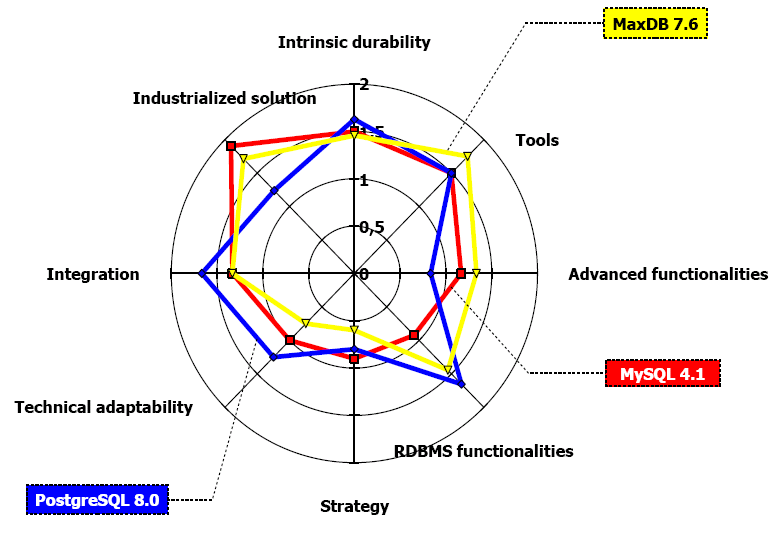
\includegraphics[height=10cm]{images/comparaison}
\caption{
Comparison. 
This figure is provided as an example, therefore weightings on the various axis are not representative of all kind of RDMBS utilisations.
}
\label{fig-comparaison}
\end{figure}

\subsection{O3S tool}
Besides implementing the strict and loose selection modes, the O3S tool also enables the consultation of data related to a specific software (ID card and evaluation criteria) and the comparison (integrally, by filtering or differentially) of software in the same family.
%Copyright (c) 2004 2005 2006 Atos Origin
%Permission is granted to copy, distribute and/or modify this
%document
%under the terms of the GNU Free Documentation License,
%      Version 1.2
%      or any later version published by the Free Software
%      Foundation;
%      with no Invariant Sections, no Front-Cover
%      Texts, and no Back-Cover
%      Texts.  A copy of the license is
%      included in the section entitled "GNU
%      Free Documentation License".
%
%$Id: internet_site.tex,v 1.1 2006/02/16 17:36:15 goneri Exp $
\section{Internet website}
The \url{http://www.qsos.org} website centralizes documents and information on the method itself and also creation, modification, certification of QSOS documents (functional grids, ID cards, evaluation sheets).



%Copyright (c) 2004 2005 2006 Atos Origin
%Permission is granted to copy, distribute and/or modify this
%document
%under the terms of the GNU Free Documentation License,
%      Version 1.2
%      or any later version published by the Free Software
%      Foundation;
%      with no Invariant Sections, no Front-Cover
%      Texts, and no Back-Cover
%      Texts.  A copy of the license is
%      included in the section entitled "GNU
%      Free Documentation License".
%
%$Id: glossary.tex,v 1.1 2006/02/16 18:21:09 goneri Exp $
\section*{Glossaire}
%\addcontentsline{toc}{chapter}{Glossaire}


\paragraph{Fork}
Un fork est un �v�nement qui appara�t parfois dans le d�veloppement
d'un projet informatique, typiquement dans des projets communautaires (cas de beaucoup
de logiciels libres), quand les opinions au sein de l'�quipe de d�veloppement divergent
sur le chemin � prendre et qu'elles ne sont pas conciliables. Le d�veloppement du
logiciel part alors dans deux directions diff�rentes, sous l'impulsion des deux camps.

\paragraph{M�thode QSOS}
M�thode de Qualification et de S�lection de logiciels Open Source, con�ue et utilis�e
par Atos Origin pour ses travaux de support et de veille technologique. Elle est mise
� disposition - sous licence libre - sur le site \url{http://www.qsos.org}.

\paragraph{O3S}
Open Source Selection Software. Outil informatique d�velopp� par Atos Origin impl�mentant la m�thode QSOS, qui sera utilis� sur le site \url{http://www.qsos.org} pour cr�er, modifier et visualiser les fiches d'identit� et d'�valuation.

\paragraph{Prestataire de services}
Toute entreprise d�sireuse d'offrir des services autour de logiciels libres ou Open Source (expertise, int�gration, d�veloppement, support, ...).

\paragraph{Utilisateur}
Toute personne physique, entit�, entreprise ou administration utilisatrice ou future utilisatrice de logiciels libres ou Open Source.




\end{document}
% vi:syntax=tex
